
\subsection{Layer preconstruction}
\label{sec:cache-design}

%In the following, we present our \sysname~\preconstructcachename design.
%Each \texttt{pull layer} request has a precedent \texttt{pull manifest} request.
%Upon receiving a \texttt{pull manifest} request, 
%\sysname~sends the updated \sysname~manifest to client.
%After receiving a \sysname~manifest, the client parses the manifest
%and sends either a \texttt{pull layer} request if the layer hasn't been deduplicated,
%or a list of \texttt{pull slice} requests if a list of corresponding slices presents in the manifest.
%Those \texttt{pull slice} requests will then be
%forwarded to all the registry servers that store the requested
%layer's slices as shown in Figure~\ref{fig:sys-overview}. 

%\begin{figure}[t]
	\centering
	\centering
	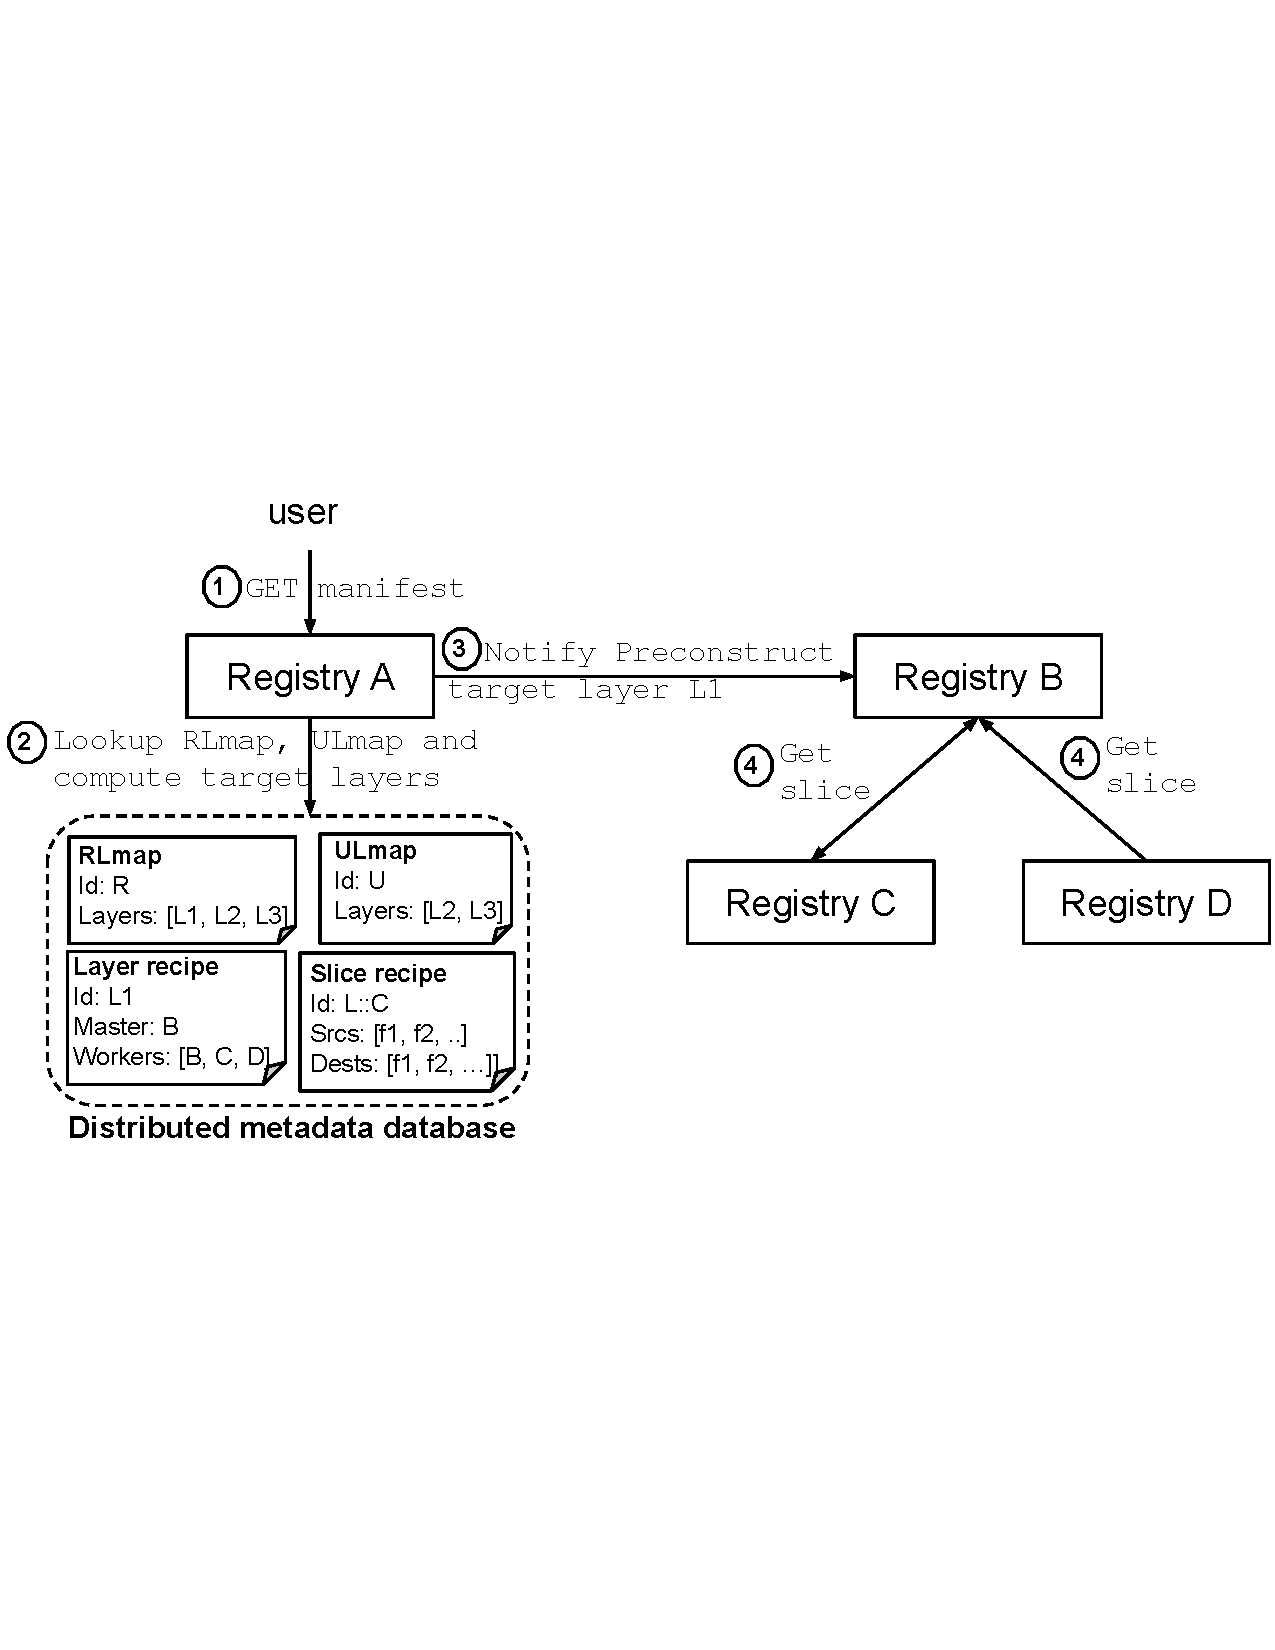
\includegraphics[width=0.49\textwidth]{graphs/sift-preconstruct.pdf}
	\caption{Layer preconstruction.}
	\label{fig:preconstruct}
\end{figure}

Based on the observations made in xxxx,
\sysname preconstructs layers before layer accesses to save layer construction time.

 After D-servers receive the backup replicas,
\sysname will first update \emph{RLmap} with the layer and its associated repository, where
RLmap maps a \textbf{repository id} (i.e., repository name) to its containing layers 
as shown in Figure~\ref{fig:dedup-partition}.

When a~\texttt{pull} layer request is received, 
\sysname will first update \emph{ULmap}. 
ULmap records user access status,
which maps a \textbf{user Id} to its accessed layers with its corresponding access count,
where user id is defined as client request address.

\paragraph{User behavior based layer preconstruction}
\begin{algorithm}
\scriptsize 
	\caption{Layer preconstruction}
	\label{alg:prefetch}
	\KwIn{\\
		$\theta_{rpc}$: Threshold for repull layers to be preconstructed. \\
		$RLmap$: Repository to layer map. \\
		$ULmap$: User to layer map.  \\
		$LayerRecipes$: Layer recipes. \\
		$SliceRecipes$: Slice recipes.\\
	}
	\emph{r} $\leftarrow$ \texttt{request received}\\
	\uIf{r = GET manifest}
		{
			difference $\gets$ \emph{RLmap[r.repo]} $-$ \emph{ULmap[r.client]} \\
			intersection $\gets$ \emph{RLmap[r.repo]} $\bigcap$ \emph{ULmap[r.client]} \\
			
			targets $\leftarrow$ difference \\
			\ForEach{layer in intersection} 
			{ \If{ layer.rpcnt $>$ $\theta_{rpc}$}{
				targets	$\leftarrow$ layer
				}
			}
			\ForEach{layer in targets} {
				master $\leftarrow$ \emph{LayerRecipes[layer].master} \\
				\texttt{Notify} master `PRECONSTRUCT layer' \\
			}
		}
	
		\uElseIf{r = PRECONSTRUCT layer}
		{
			\If{r.layer not in DiskCache}{
				workers $\leftarrow$ \emph{LayerRecipes[r.layer].workers} \\
				\ForEach{worker in workers} {
					%{\scriptsize $/*$\textit{sliceid = r.layer+worker}}\\ 
					slices $\leftarrow$ \texttt{GET slice from} worker `GET slice' \\
				}
				layer $\leftarrow$ \texttt{Concatenate} slices \\
				
				DiskCache $\gets$ layer \\
				{\tiny{$/*$\texttt{Set timer for layer}} $/*$}\\
			}
		}
	
		\uElseIf{r = GET slice}
		{
			slice $\leftarrow$ \texttt{Construct by following} \emph{SliceRecipes[r.slice]} \\
			
			\texttt{Serve} slice \\
		}
	
%		\uElseIf{r = PUT layer}
%		{
%				\emph{LayerCache} $\leftarrow$ \texttt{cache} \emph{r.layer} \\
%				\texttt{update} \emph{RLmap[r.repo, r.layer]} \\
%		}
%		\uElseIf{r = GET layer} 
%		{
%			{\tiny\texttt{/* r.layer has not been deduplicated   /}} \\
%				\eIf{r.layer in cache}
%				{
%					\emph{cache hit for layer} \\
%					\texttt{Serve} layer \\
%				} 
%				{
%					workers $\leftarrow$ \emph{LayerRecipes[layer].workers} \\
%					\ForEach{slave in slaves} {
%						slices $\leftarrow$ \texttt{GET} worker `GET layer'slice' \\
%					}
%					layer $\leftarrow$ \texttt{Concatenate} slices \\
%					\texttt{Serve} layer
%					LayerCache $\gets$ layer \\
%				}
%		}
%		\texttt{update} \emph{ULmap[r.client, r.repo, r.layer]} \\
		
\end{algorithm}




Figure~\ref{fig:preconstruct}
shows how to preconstruct layers for later accesses.
When a \texttt{GET manifest} request is received by registry $A$,
it gets the requested repository information and client information from RLmap and ULmap respectively, 
and computes a list of target layers that will be accessed later by this client.
As shown, to preconstruct target layer $L1$, 
registry $A$ gets $L1$'s layer recipe from metadata database
and sends a notification of \texttt{preconstruct layer} $L1$ to 
$L1$'s restoring master: registry $B$. 
After receiving the notification, 
$B$ sends \texttt{get slice} requests to its peer workers: $C$ and $D$.
When $B$, $C$, and $D$ finished slice constructions for $L$,
three slices are concatenated by $B$ and saved in $B$'s layer diskcache. 

Algorithm~\ref{alg:prefetch} shows how to determine target layers 
based on observed user access pattern.
When a \texttt{GET manifest} request \emph{r} is received,
\sysname~gets a set of layers associated with the requested repository \emph{r.repo} from RLmap, 
denoted as $RLmap[r.repo]$.
Meanwhile, it also gets a set of layers associated with the client \emph{r.client} from ULmap,
denoted as $ULmap[r.client]$.
After that, it calculates a list of layers in the requested repository 
that have not been \texttt{pulled} by the client by
computing the difference set between $RLmap[r.repo]$ and $ULmap[r.client]$ (denoted as $difference$).
All the layers in $difference$ are included in target set.
\sysname also calculates a intersection set between 
$RLmap[r.repo]$ and $ULmap[r.client]$ (denoted as $intersection$).
The layers in $intersection$ are already pulled by client.
To determine whether a layer in $intersection$ will be
$repulled$ by client,
\sysname compares its repull count against a predefined threshold $\theta_{rpc}$.
If the layer's repull count is greater than $\theta_{rpc}$,
which means this layer will be repulled with high probability.
Thus, it is included in target layer set.

For each layer in target set, 
\sysname gets the restoring master from its layer recipe,
and sends a notification of \texttt{preconsturct layer} to the master.
After the master receives the notification,
it first checks if the requested layer is in the preconstruct cache.
If not, 
it starts layer construction and saves the preconstructed layer in the preconstruct cache.
 
%and gets two groups of layers: \emph{newLayers} and \emph{oldLayers}.
%\emph{newLayers} means the layers that belongs to \emph{r.repo} but haven't been pulled by client \emph{r.client}.
%While \emph{oldLayers} means the layers that belongs to both of them.
%\preconstructcachename~will first restore the slices for \emph{newLayers} because 
%they are not locally available to \emph{r.client}.    
%For \emph{oldLayers}, 
%if an \emph{oldLayer} has a higher repull count and \emph{r.repo} as well as \emph{r.client} have a higher repulling probability,
%then \preconstructcachename~will restore its slices and cache them.
%If a \emph{PUT} layer request is received, RLmap and URLmap will be updated accordingly.
%
%If a \emph{GET} layer request is received, it means that \emph{r.layer} has not been deduplicated.
%\preconstructcachename~will cache \emph{r.layer} if cache miss happens on \emph{GET} layer request as shown in Algorithm~\ref{alg:prefetch}.
%If a \emph{GET} slice request is received, meaning that \emph{r.layer} has already been deduplicated into deduplicated slices,
%\preconstructcachename~will check if the requested \emph{r.slice} exists in the cache.
%If not,
%\dedupname system~will start restoring \emph{r.slice} and also put it in cache.
%In the end, \preconstructcachename~will update URLmap with corresponding repull count and repull probability.
\paragraph{Preconstruct cache eviction}
To exploit the temporal trend of clients and repositories, 
\sysname sets timer for each cached layers.
Once a layer is expired,
it will be simply deleted from the preconstruct cache.

Preconstruct cache replacement is triggered when the free space in the cache is
lower than threshold $\theta_{C}$.
As shown in Algorithm~\ref{alg:eviction}, 
\sysname~maintains a LFRU list~\cite{xxx} of cached layers to exploit 
layer temporal trend.
If the free space is low,
\sysname~selects the least frequent recently used layer to evict.



\begin{algorithm}
	\scriptsize 
	\caption{User access history based eviction.}
	\label{alg:eviction}
	\SetAlgoLined
	\KwIn{\\
		$T_{mem}$: Capacity threshold for MEM cache to trigger demotion. \\
		$T_{flash}$: Capacity threshold for FLASH cache to trigger eviction. \\
		$UsrLRU$: LRU of users.  \\
		$LayerLRU[Usr]$: LRU of layers that are accessed by user $Usr$. \\
		$RepoLRU$: LRU of repostiories. \\
		$LayerLRU[Repo]$: LRU of layers that are associated with repository $Repo$.
	}
	\While{free\_MEM $<$ $T_{mem}$}{
		\emph{last\_usr} $\gets$ \emph{UsrLRU.last\_item()}\\
		\For{last\_layer $\gets$ \emph{LayerLRU[last\_usr].last\_item()}}{
			\If{layer exclusively belongs to last\_usr}{
				%{\scriptsize $/*$\textit{If layer is not shared with other users, layer is deleted}}\\
			%	last\_layer $\gets$ \emph{LayerLRU[last\_usr]}\\			
				FLASHcache $\gets$ \emph{Demote(last\_layer)} \\
				\emph{free\_MEM} $+=$ \emph{sizeof(last\_layer)} \\
			}
		}
	}

	\While{free\_FLASH $<$ $T_{flash}$}{
	\emph{last\_repo} $\gets$ \emph{RepoLRU.last\_item()}\\
	\For{last\_layer $\gets$ \emph{LayerLRU[last\_repo].last\_item()}}{
		\If{layer exclusively belongs to last\_repo}{
			%{\scriptsize $/*$\textit{If layer is not shared with other users, layer is deleted}}\\
			%	last\_layer $\gets$ \emph{LayerLRU[last\_usr]}\\			
			\emph{Discard(last\_layer)} \\
			\emph{free\_FLASH} $+=$ \emph{sizeof(last\_layer)} \\
		}
	}
}

\end{algorithm}


%\begin{algorithm}
%    \tiny 
%	\caption{User access history based eviction}
%	\label{alg:prefetch}
%	%\SetAlgoLined
%	\KwIn{\\
%		$L_{thresh}$: Threshold for duration to keep a prefetched layer. \\
%		$RLMap$: Repository to layers map.\\
%		$URLMap$: User to layers map. \\
%	}
%	\While{true}{
%		\emph{r} $\leftarrow$ \texttt{request received}\\
%		\uIf{r = GET manifest}
%		{
%%			layerlst $\leftarrow$ URLMap[(r.client, r.repo)]
%			\emph{layers} $\gets$ \emph{RLMap[r.repo]} $-$ \emph{URLMap[r.client]} \\
%			\emph{OnTimelayers}, \emph{NotOnTimelayers} $\gets$ \emph{OnTimeCalculation(layers)} \\
%			\emph{MEMcache} $\gets$ \emph{Prefetch(OnTimelayers)} \\
%			\emph{FLASHcache} $\gets$ \emph{Prefetch(NotOnTimelayers)} \\
%			\texttt{set} \emph{L\_timer[layer] for each layer in layer} \\
%			{\tiny\texttt{/*when $L\_timer[layer] > L\_thresh$, layer is evicted/}}
%			}
%		\uElseIf{r = PUT layer }
%		{
%				\texttt{update} \emph{URLMap[(r.client, r.layer)]} \\
%				\texttt{update} \emph{RLMap[(r.repo, r.layer, put)]} \\
%				\emph{MEMcache} $\leftarrow$ \texttt{buffer} \emph{r.layer} \\
%				\texttt{set} \emph{L\_PUT\_timer[r.layer]} \\
%				{\tiny\texttt{/*when $L\_timer[layer] > L\_thresh$, layer is evicted/}}	 \\
%			}
%		\ElseIf{r = GET layer}
%		{
%				\eIf{r.layer in MEMcache or r.layer in FLASHcache}
%				{
%					\emph{serve from MEMcache or FLASHcache} \\
%					\texttt{update} \emph{URLMap[(r.client, r.layer)]} \\
%					\texttt{Reset} \emph{L\_timer[r.layer]}\\
%					\emph{hit++} 
%				}
%			   {
%					\emph{serve from backend storage system} \\
%					\texttt{update} \emph{URLMap[(r.client, r.layer, repulled)]} \\
%					\emph{RepulledLayers} $\gets$ \emph{RLMap[r.repo]} \\
%					\emph{FLASHcache} $\gets$ \emph{Prefetch(RepulledLayers)} \\
%					\texttt{set} \emph{L\_timer[layer] for each layer in layers} \\
%					{\tiny\texttt{/*when $L\_timer[layer] > L\_thresh$, layer is evicted/}}
%			}
%		}
%	}
%\end{algorithm}

%%\begin{figure*}[t]
%		\begin{minipage}{0.32\linewidth}
%			\centering
%			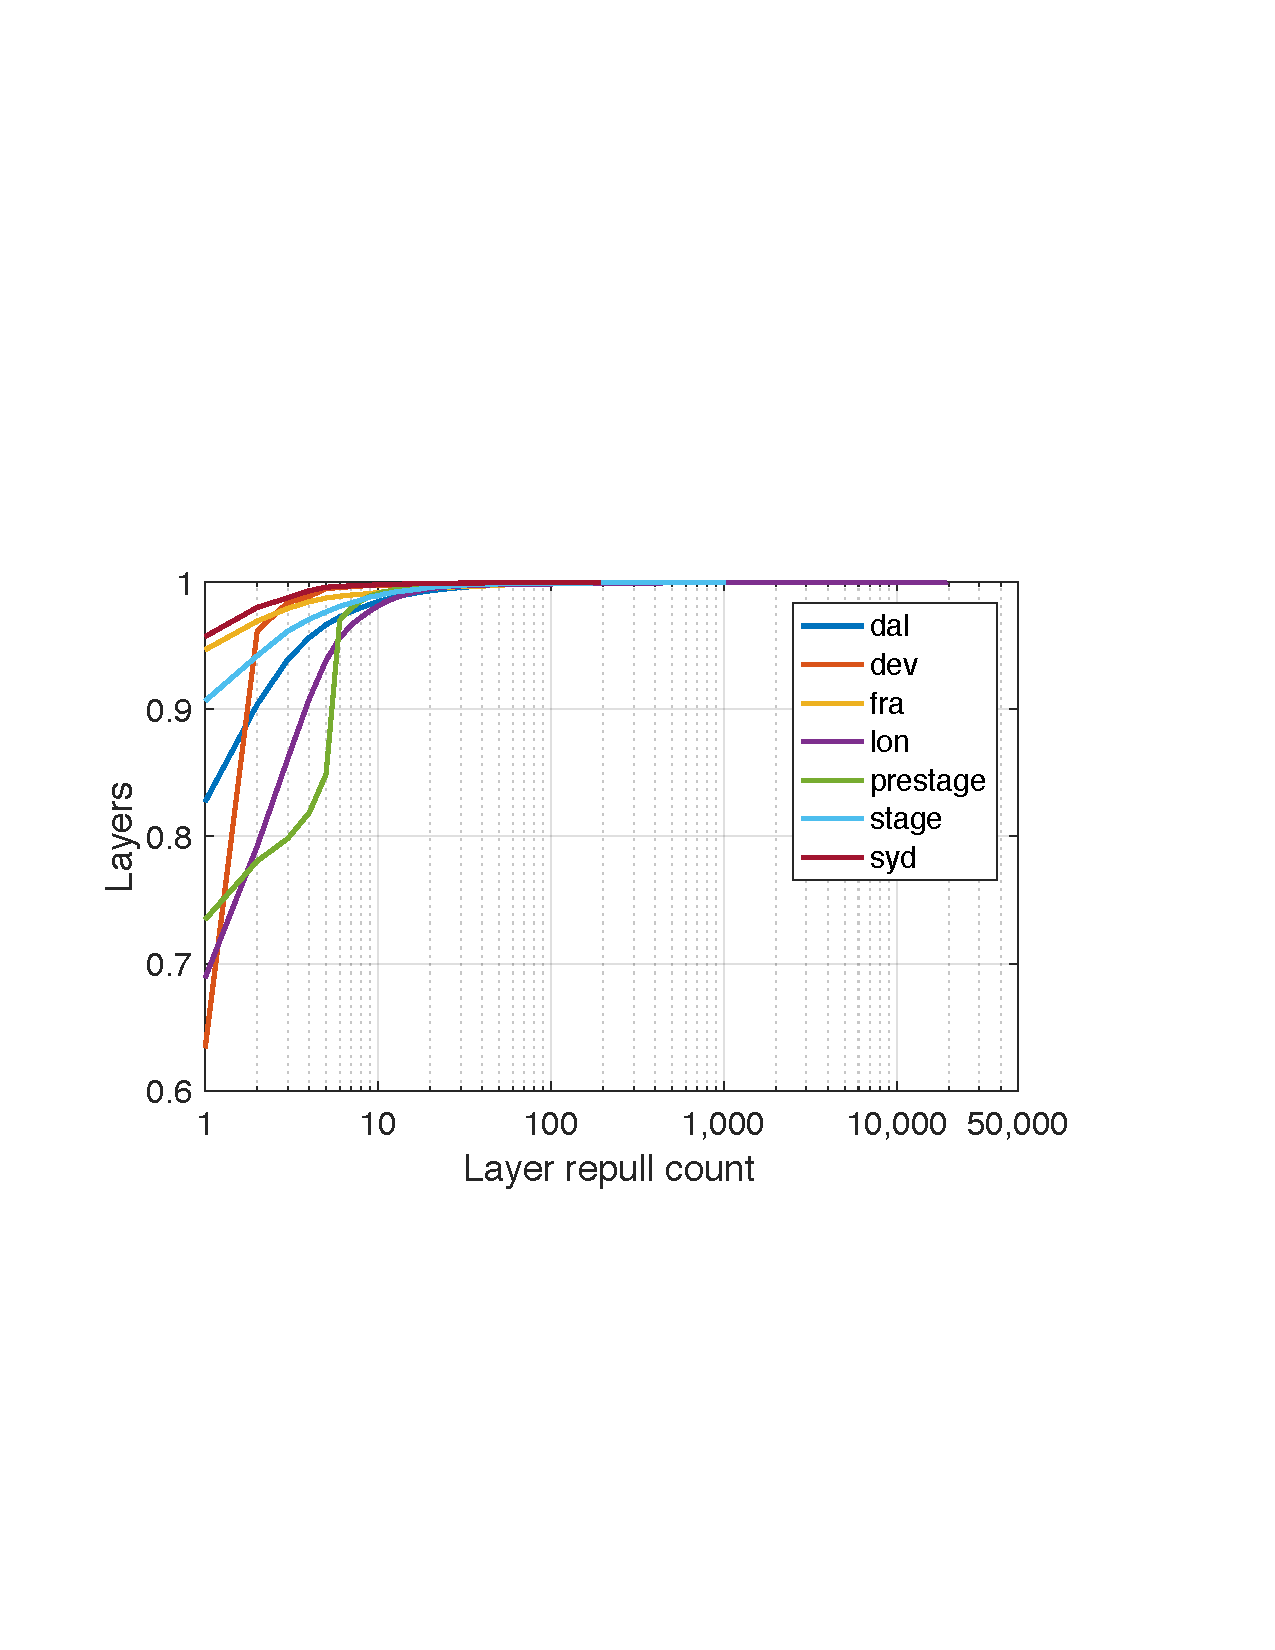
\includegraphics[width=1\textwidth]{graphs/cdf-layer-repull-by-same-client.pdf}
%			%\caption{CDF of layer repull count.}
%		%	\vspace{-3pt}
%			\label{fig:layer-repull-cdf}
%		\end{minipage}
%			\begin{minipage}{0.32\linewidth}
%				\centering
%				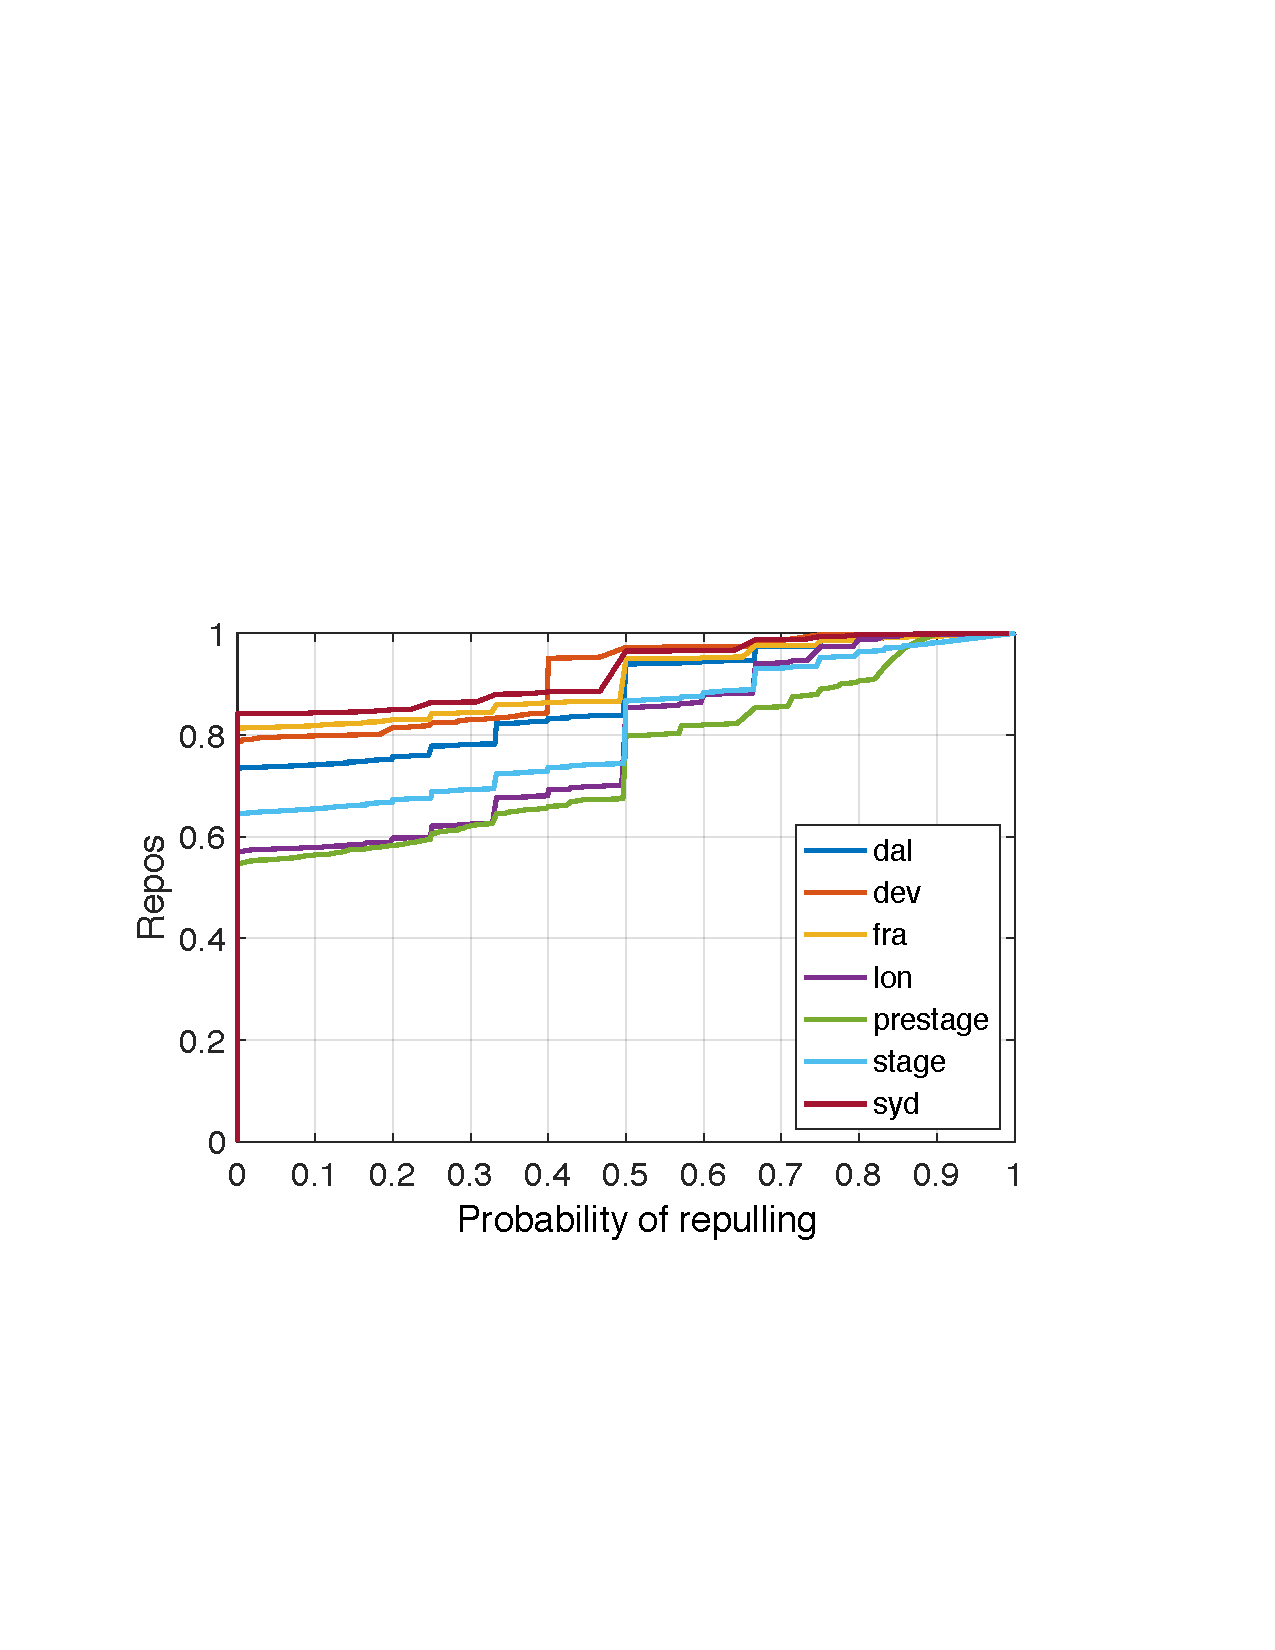
\includegraphics[width=1\textwidth]{graphs/cdf-repo-repull-ratio-by-same-client.pdf}
%				%\caption{PDF of repository repulling probability.}
%				%	\vspace{-3pt}
%				\label{fig:repo-repull-cdf}
%			\end{minipage}
%		\begin{minipage}{0.32\linewidth}
%			\centering
%			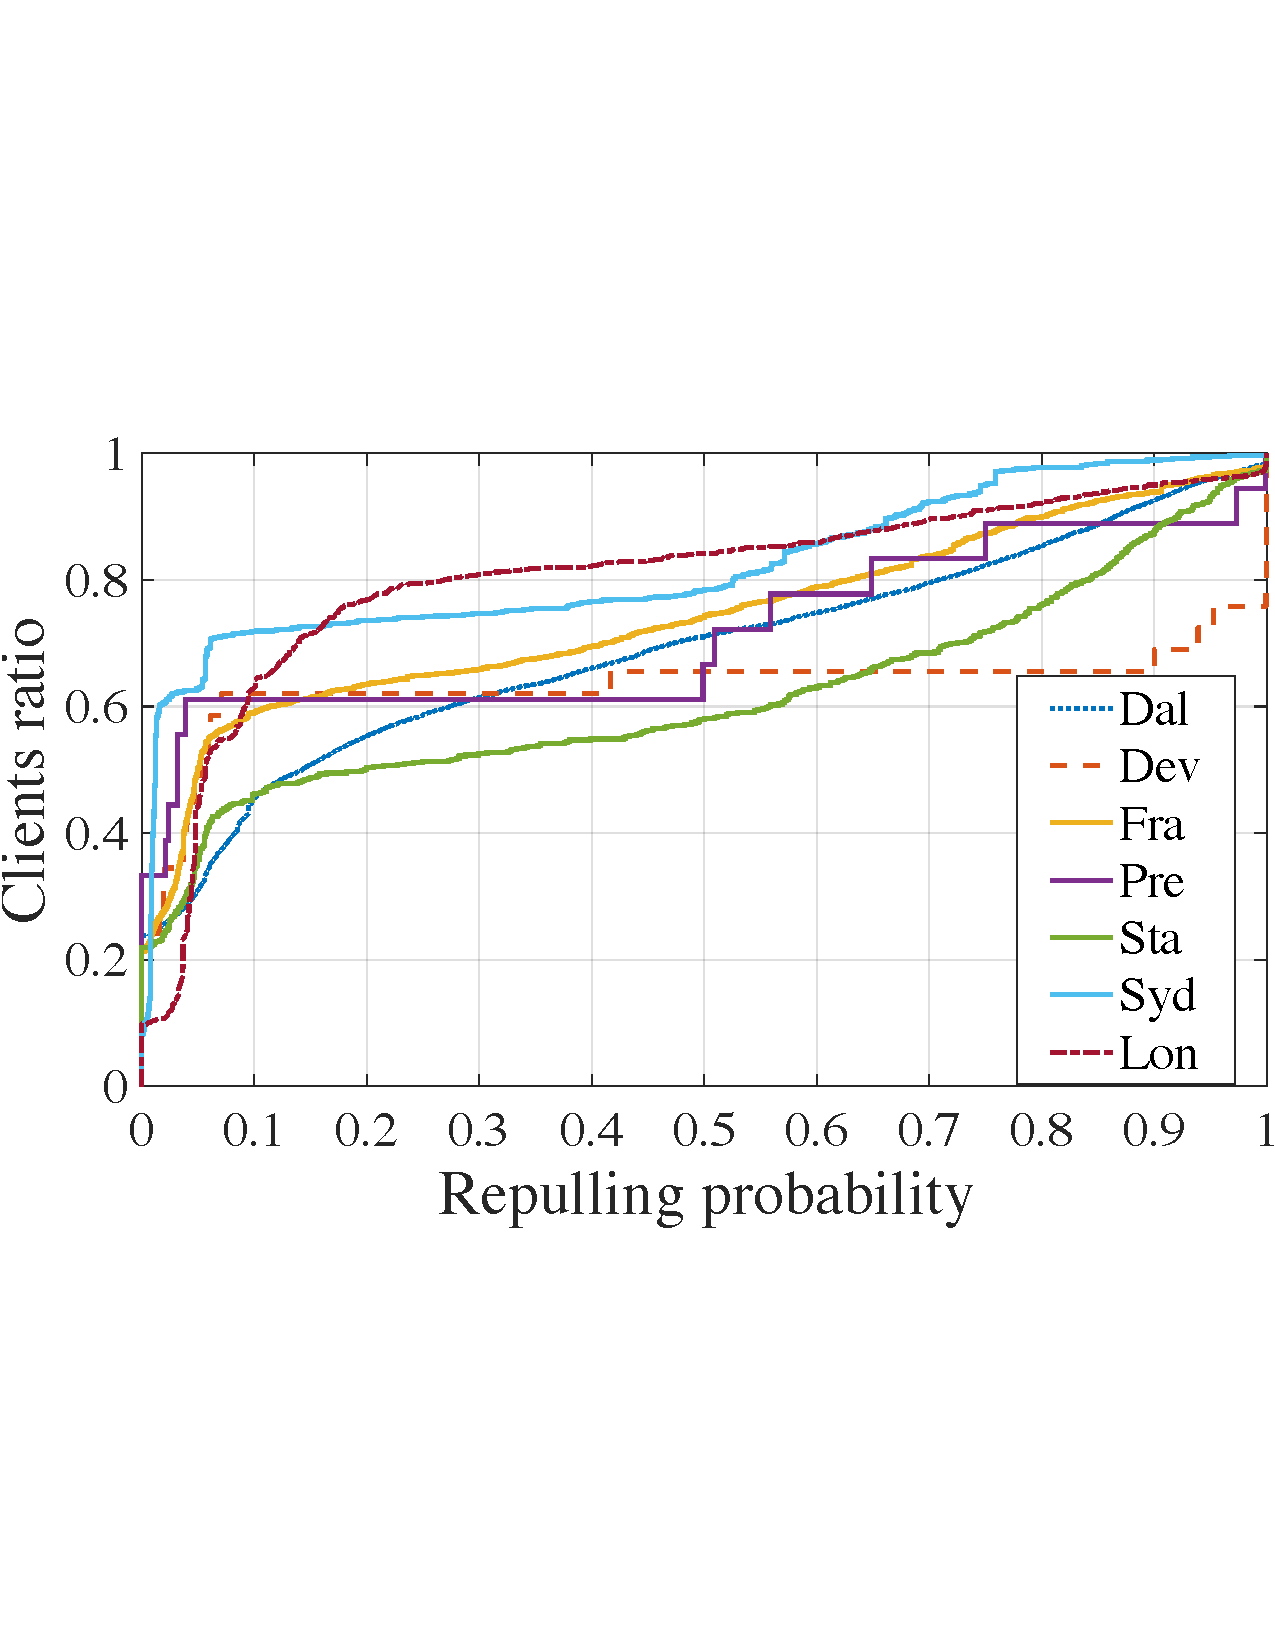
\includegraphics[width=1\textwidth]{graphs/cdf-client-repull-layer-request-ratio.pdf}
%			%
%			%	\vspace{-3pt}
%			\label{fig:client-repull-cdf}
%		\end{minipage}
%	\caption{PDF of client repull count, repository repulling probability, and client repulling probability..}
%\end{figure*}

%\begin{figure}[!t]
%	\centering
%	\subfigure[\texttt{GET} layer request count]{
%		\includegraphics[width=0.22\textwidth]{graphs/cdf-layer-repull-ratio-by-same-client.pdf}
%		\label{fig:layer-repull-cdf}
%	}
%%	\subfigure[Repository repulling probability]{
%%		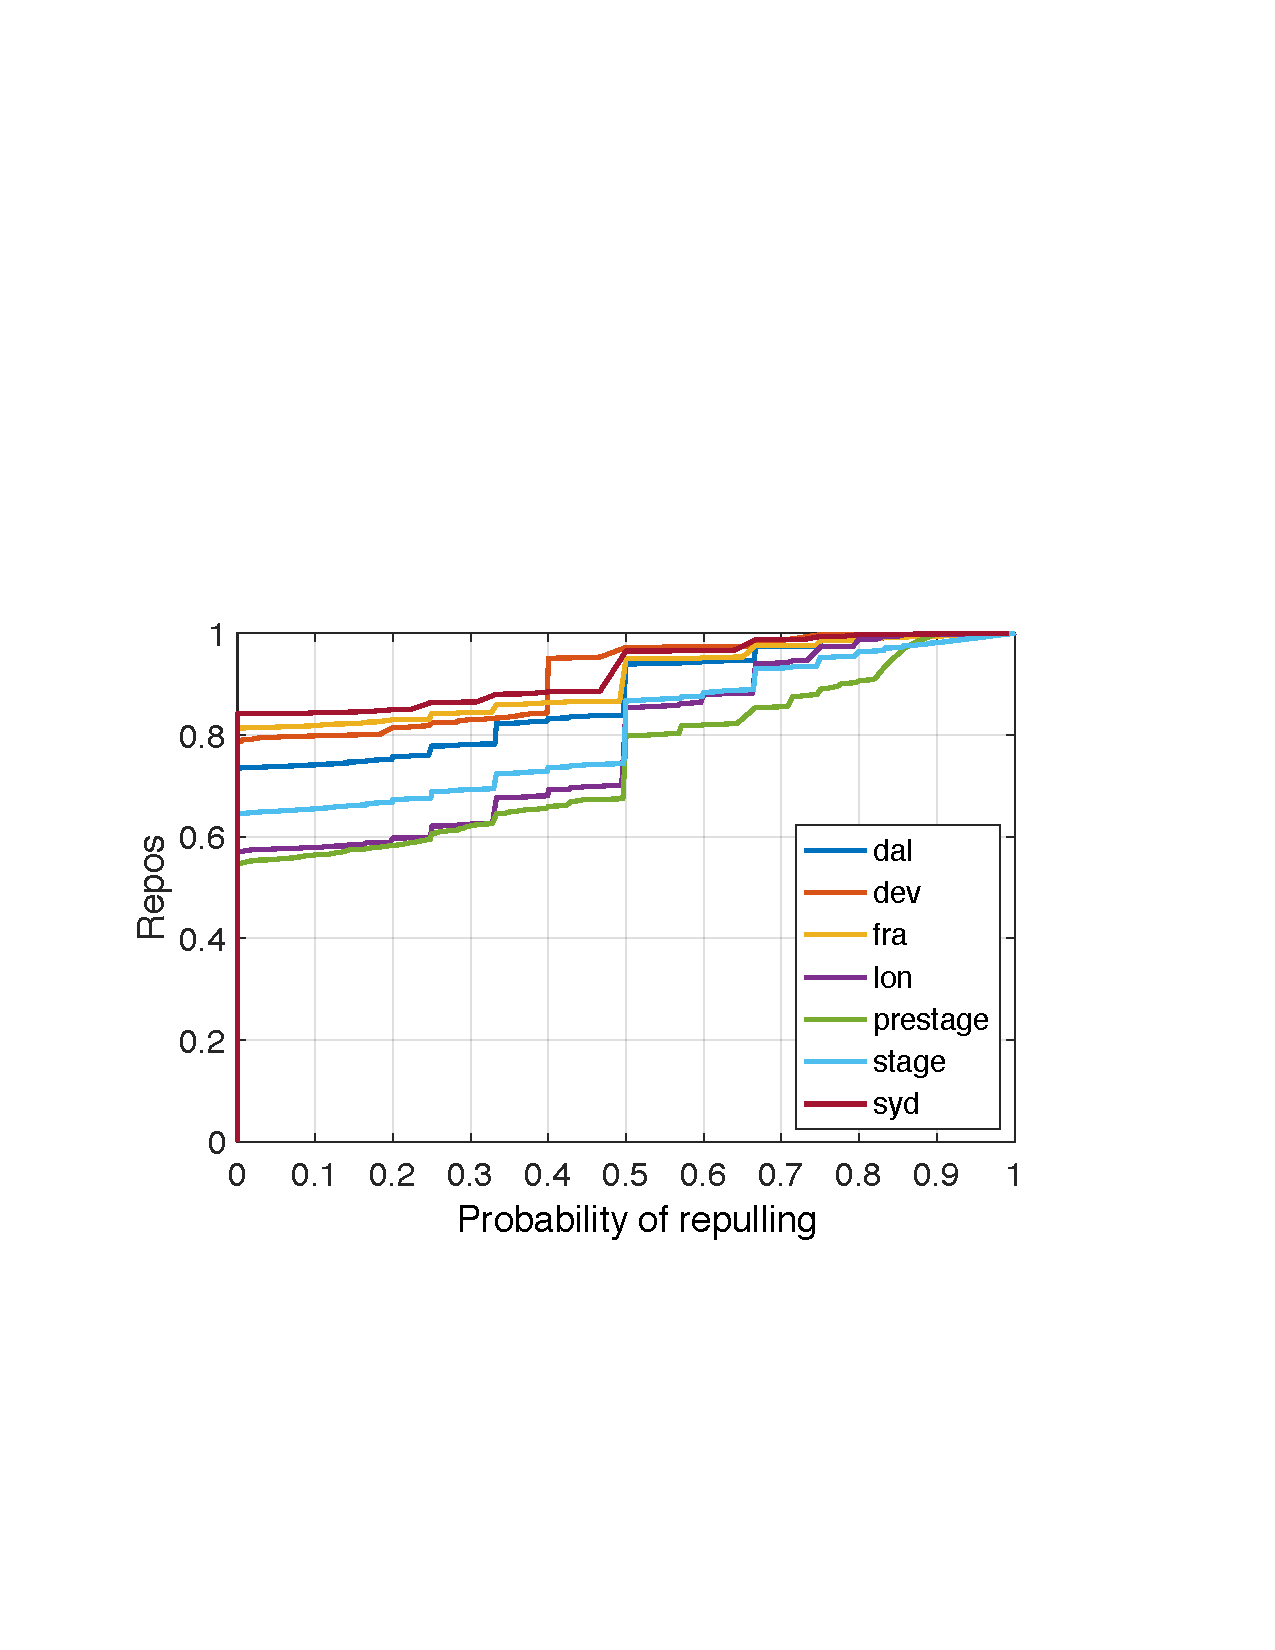
\includegraphics[width=0.2\linewidth]{graphs/cdf-repo-repull-ratio-by-same-client.pdf}
%%		\label{fig:repo-repull-cdf}
%%	}
%	\subfigure[Client repulling probability]{
%	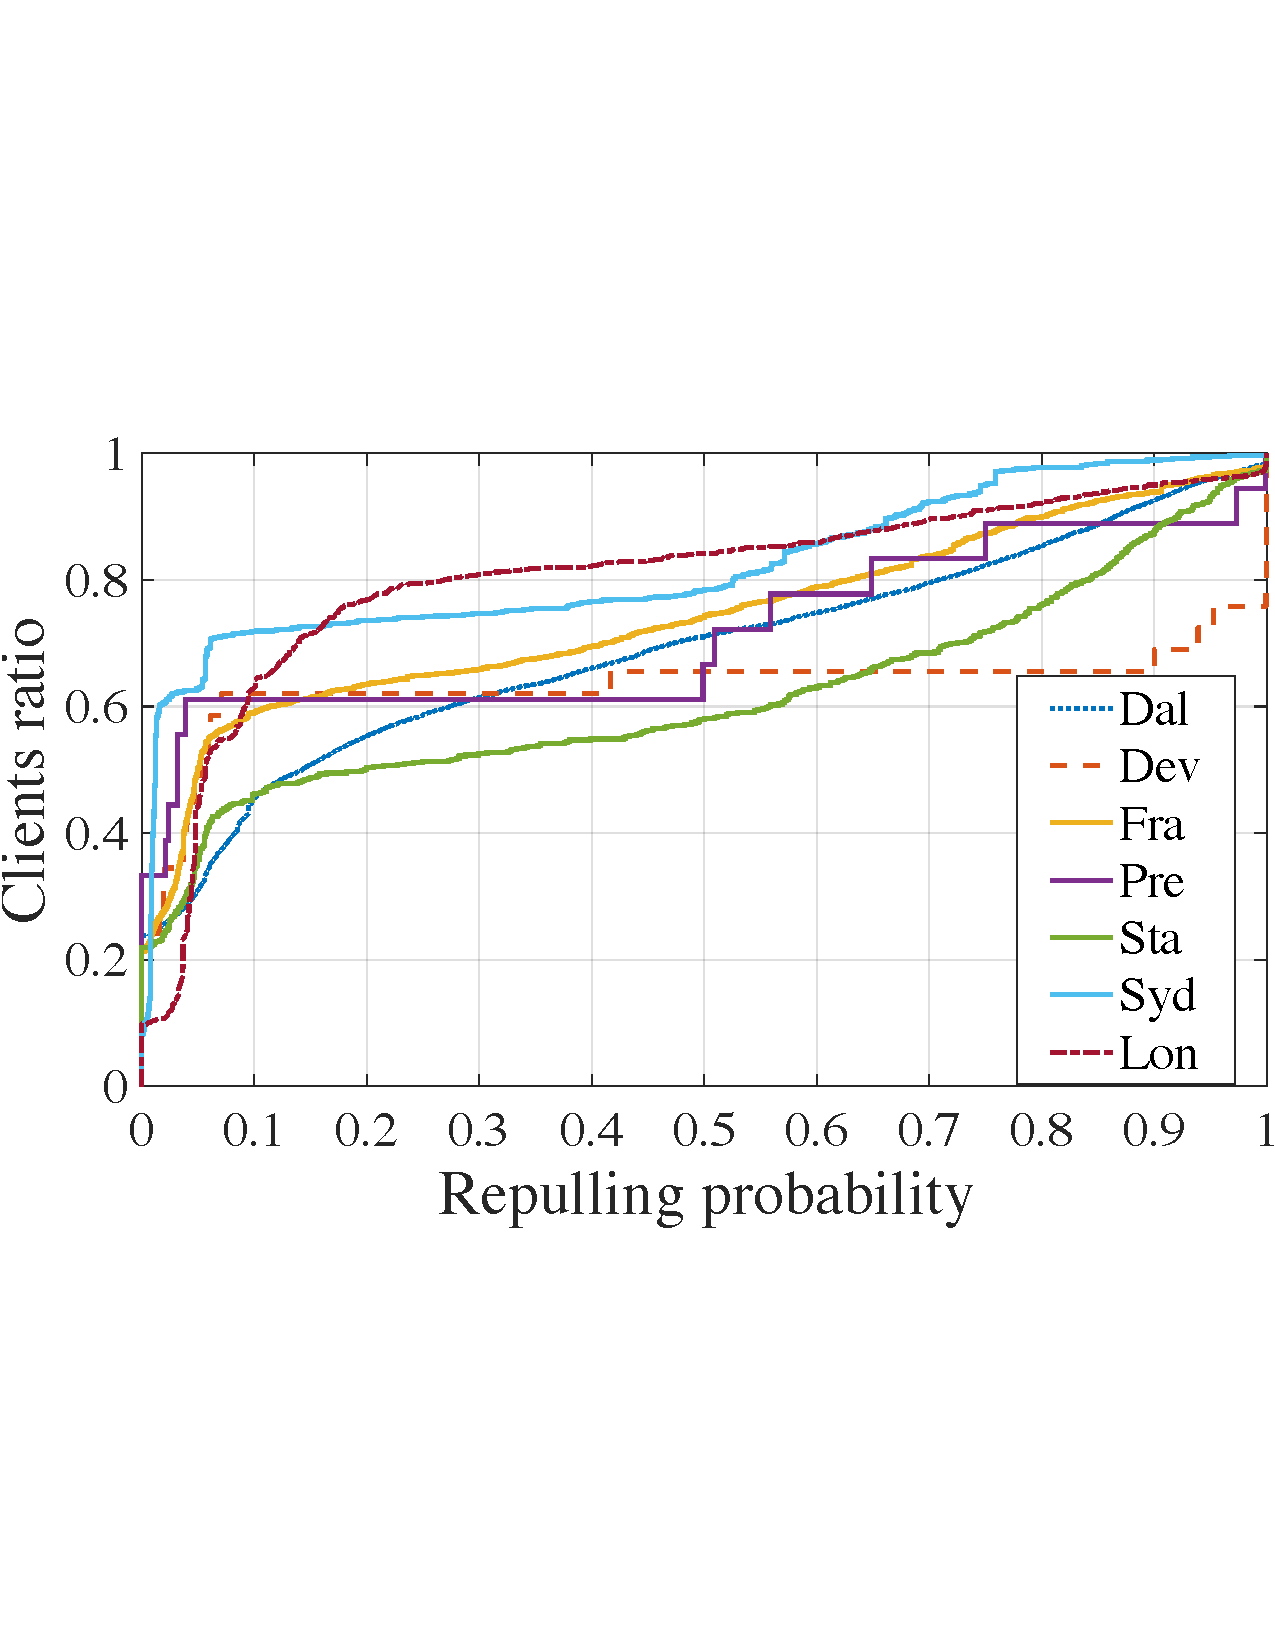
\includegraphics[width=0.2\textwidth]{graphs/cdf-client-repull-layer-request-ratio.pdf}
%   \label{fig:client-repull-cdf}
%}
%	\caption{CDF of \texttt{GET} layer request count and client repulling probability.}
%	\label{fig-repull}
%\end{figure}
%






\begin{figure*}[t]
        \centering
        \begin{minipage}{0.3\textwidth}
                \centering
                \includegraphics[width=0.9\textwidth]{{graphs/cdf-layer-repull-ratio-by-same-client.pdf}
                \caption{CDF of \texttt{GET} layer request count}
                \label{fig:layer-repull-cdf}
        \end{minipage}%
        \begin{minipage}{0.3\textwidth}
                \centering
                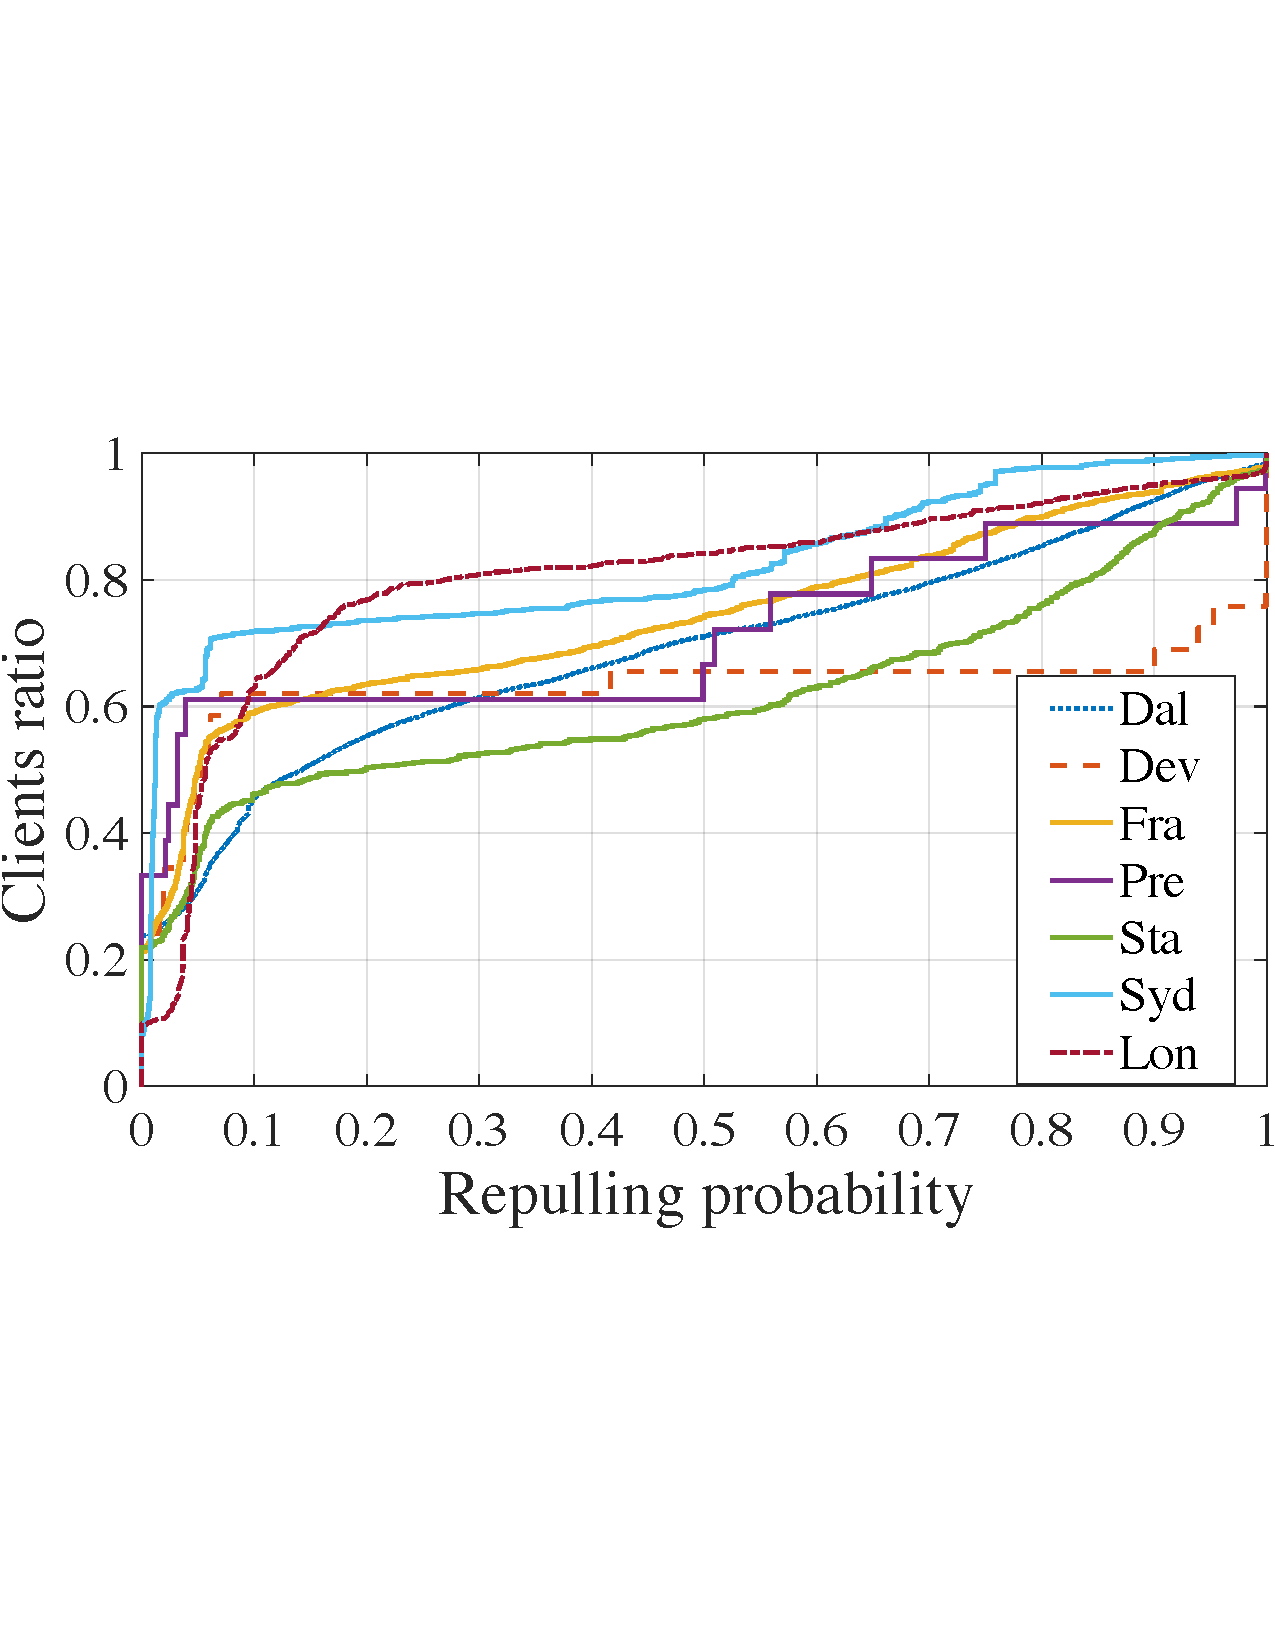
\includegraphics[width=0.9\textwidth]{graphs/cdf-client-repull-layer-request-ratio.pdf}
                \caption{CDF of Client repulling probability}% of LRU cache and preconstruct cache.}
                \label{fig:client-repull-cdf}
        \end{minipage}%
        \begin{minipage}{0.3\textwidth}
        \centering
        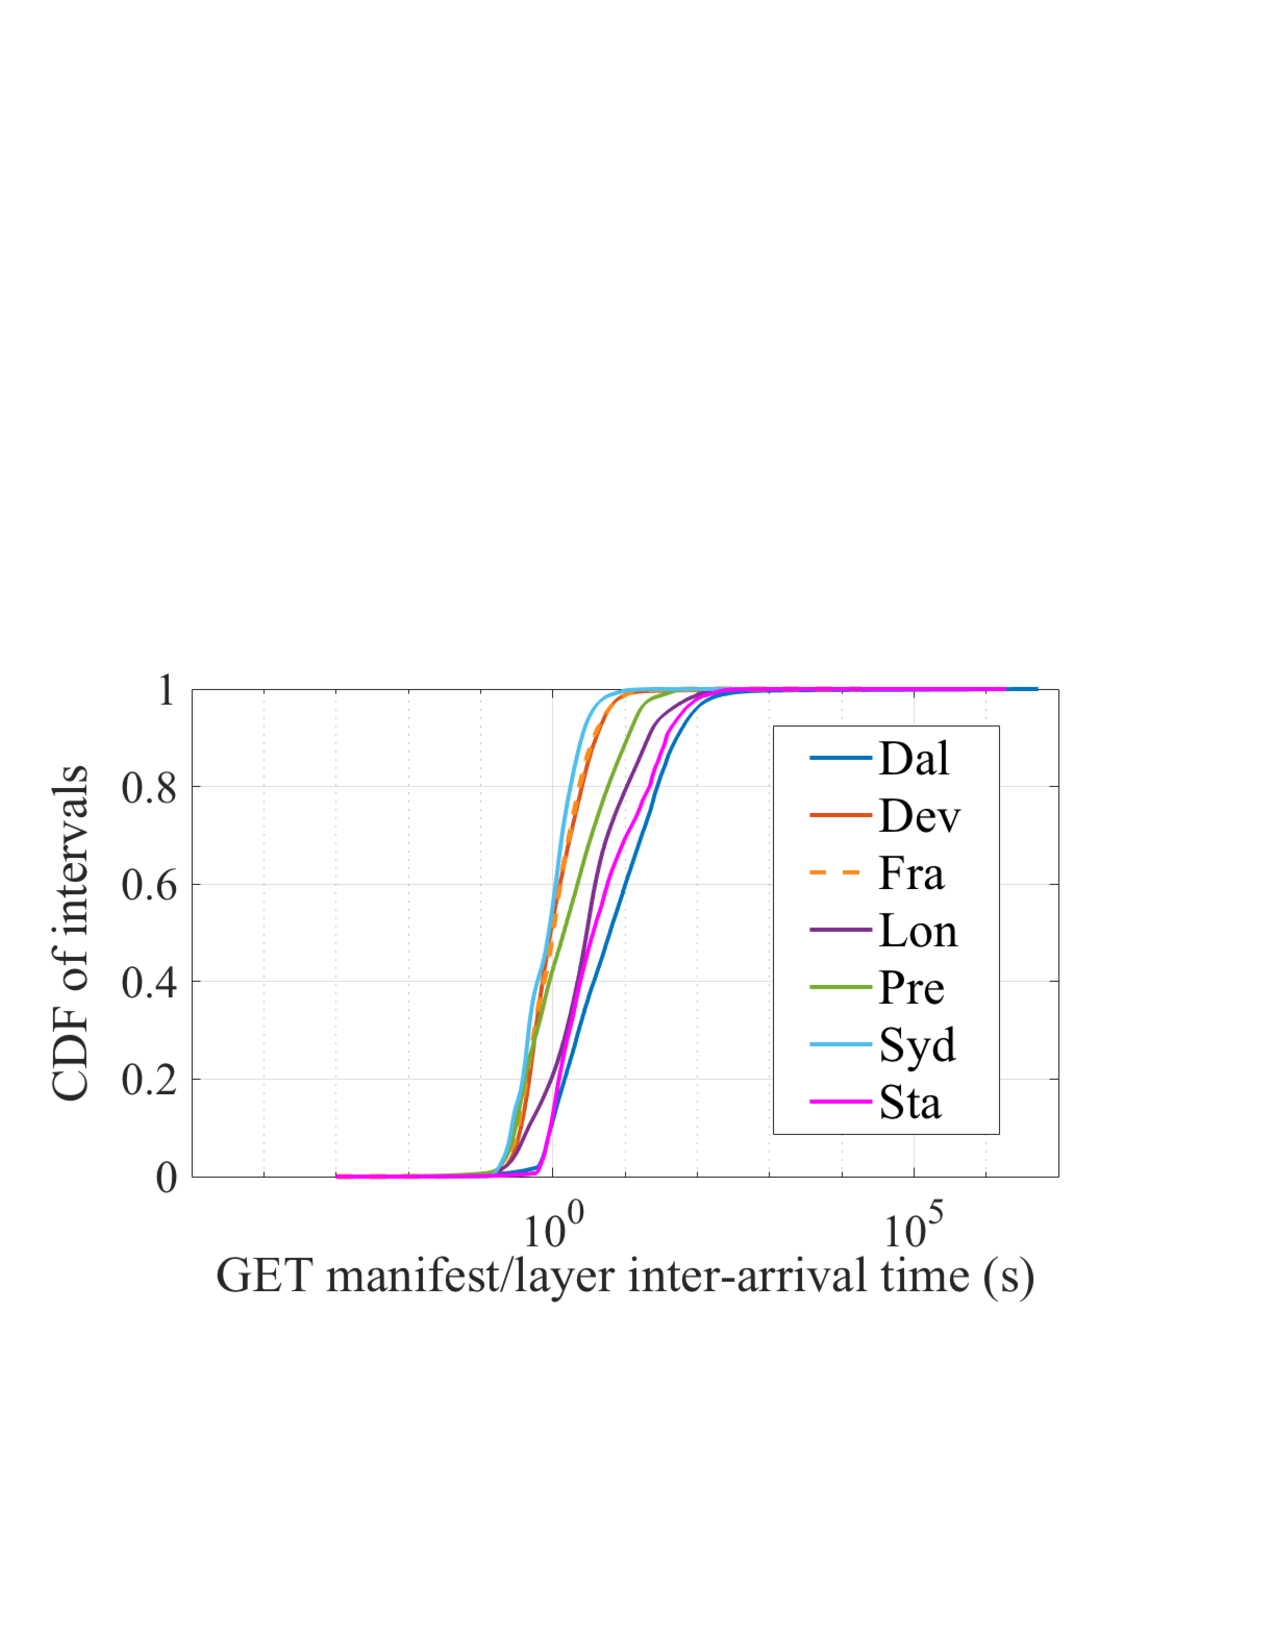
\includegraphics[width=0.9\textwidth]{graphs/GML-intervals.pdf}
        \caption{Intervals between \texttt{GET} manifest request and \texttt{GET} layer request}
        \label{fig:intervals}
   \end{minipage}
\end{figure*}





%\begin{figure}[!t]
%	\centering
%	\subfigure[CDF of compression ratio]{\label{fig_cdf_compression_ratio}
%		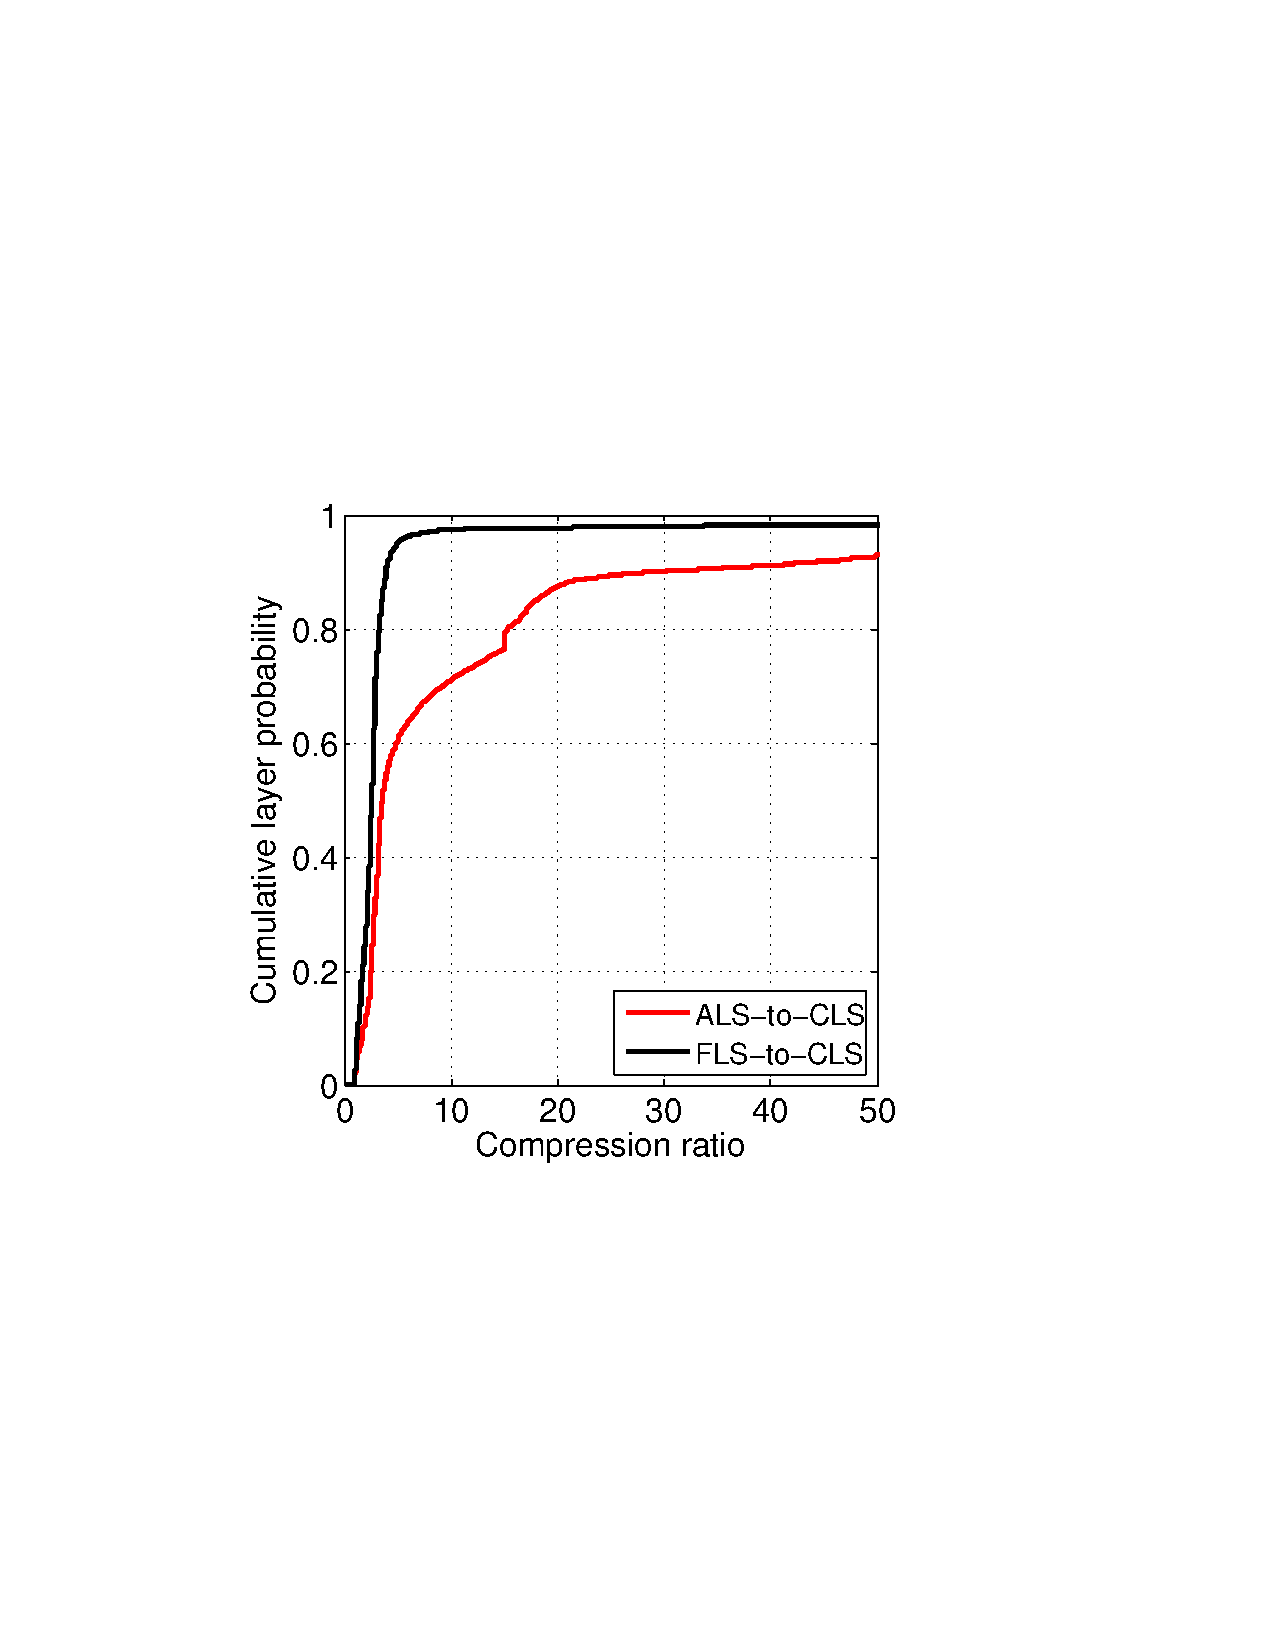
\includegraphics[width=0.23\textwidth]{graphs/cdf_compression_ratio.pdf}
%	}
%	\subfigure[Histogram of comp. ratios]{\label{fig_his_compression_ratio}
%		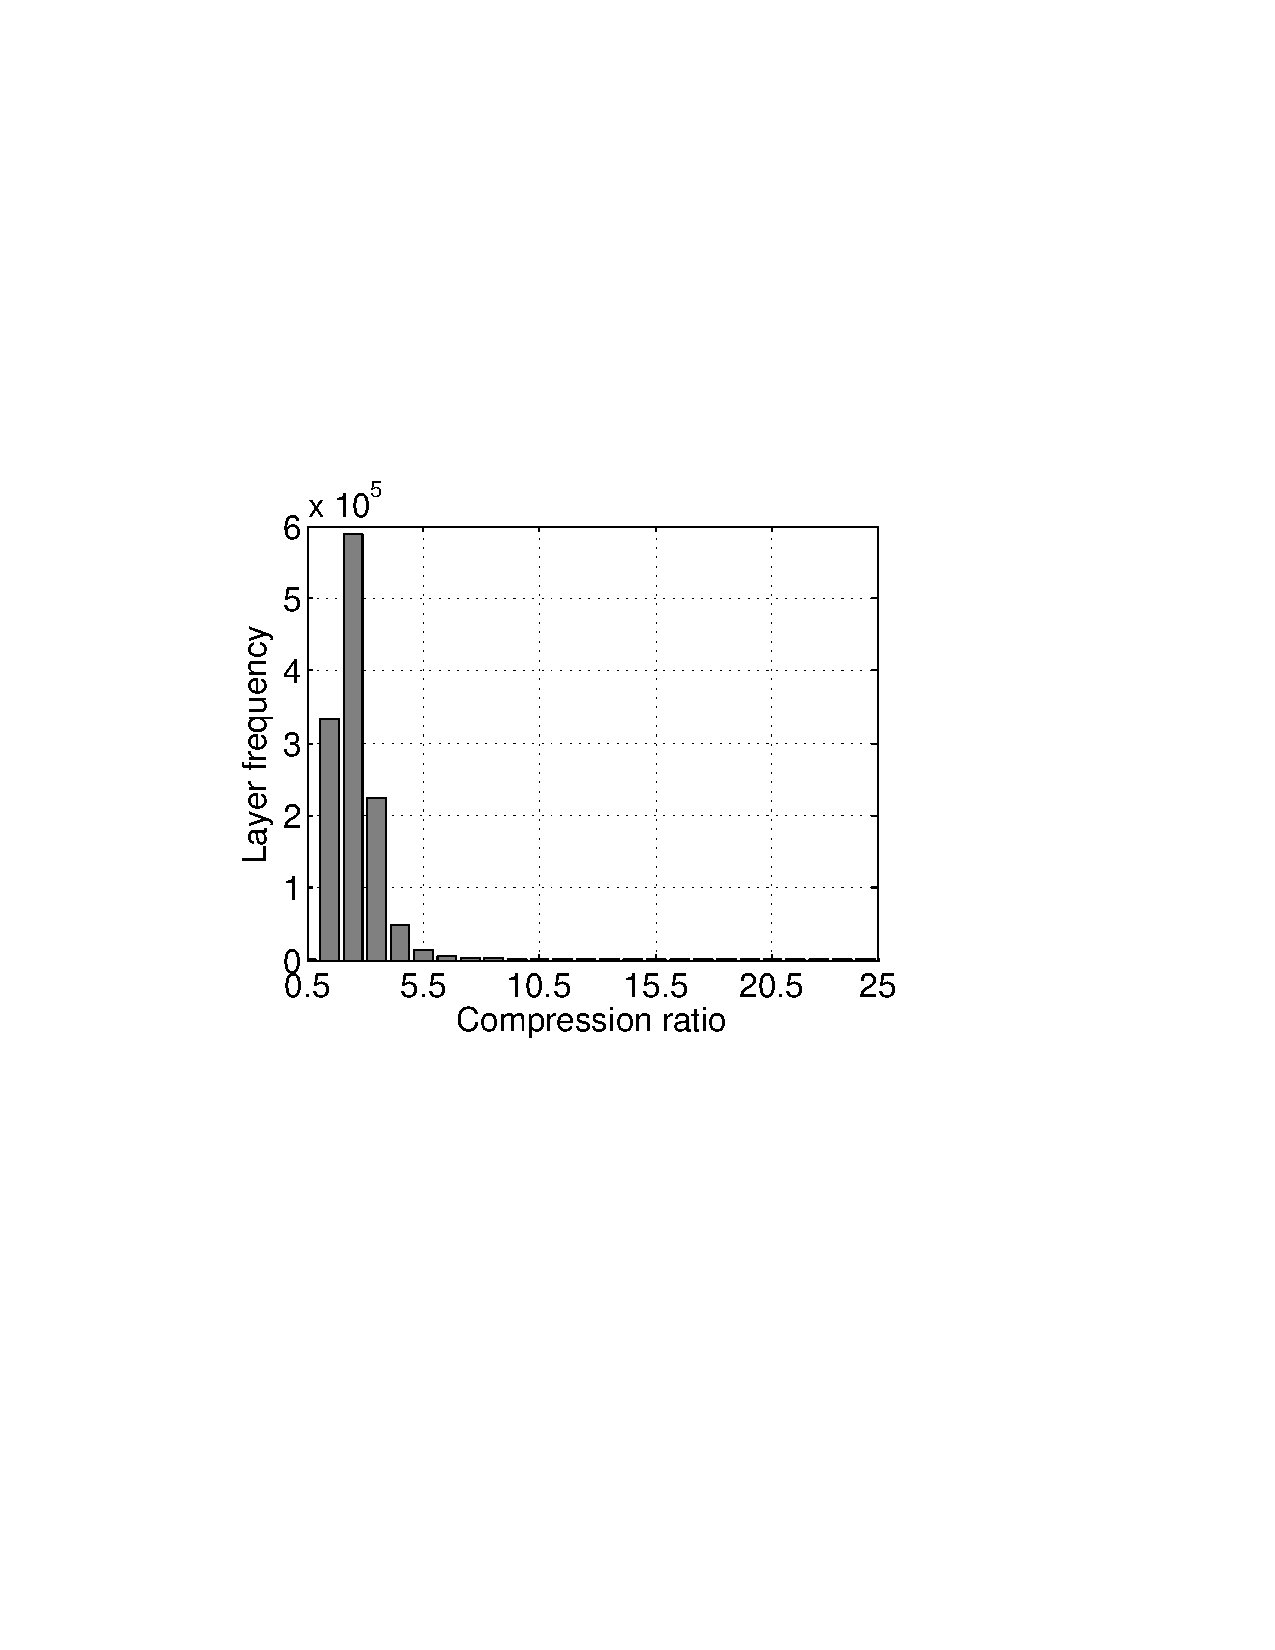
\includegraphics[width=0.223\textwidth]{graphs/his_compression_ratio.pdf}
%	}
%	\caption{Layer compression ratio distribution
%		%\vcomment{Different colors are used in figure (a) and (b) FLS/CLS\nancomment{will address later}}
%	}
%	\label{fig-compression-ratio}
%\end{figure}


%\begin{figure}[t]
%	\centering
%	\begin{minipage}{0.26\textwidth}
%		\centering
%		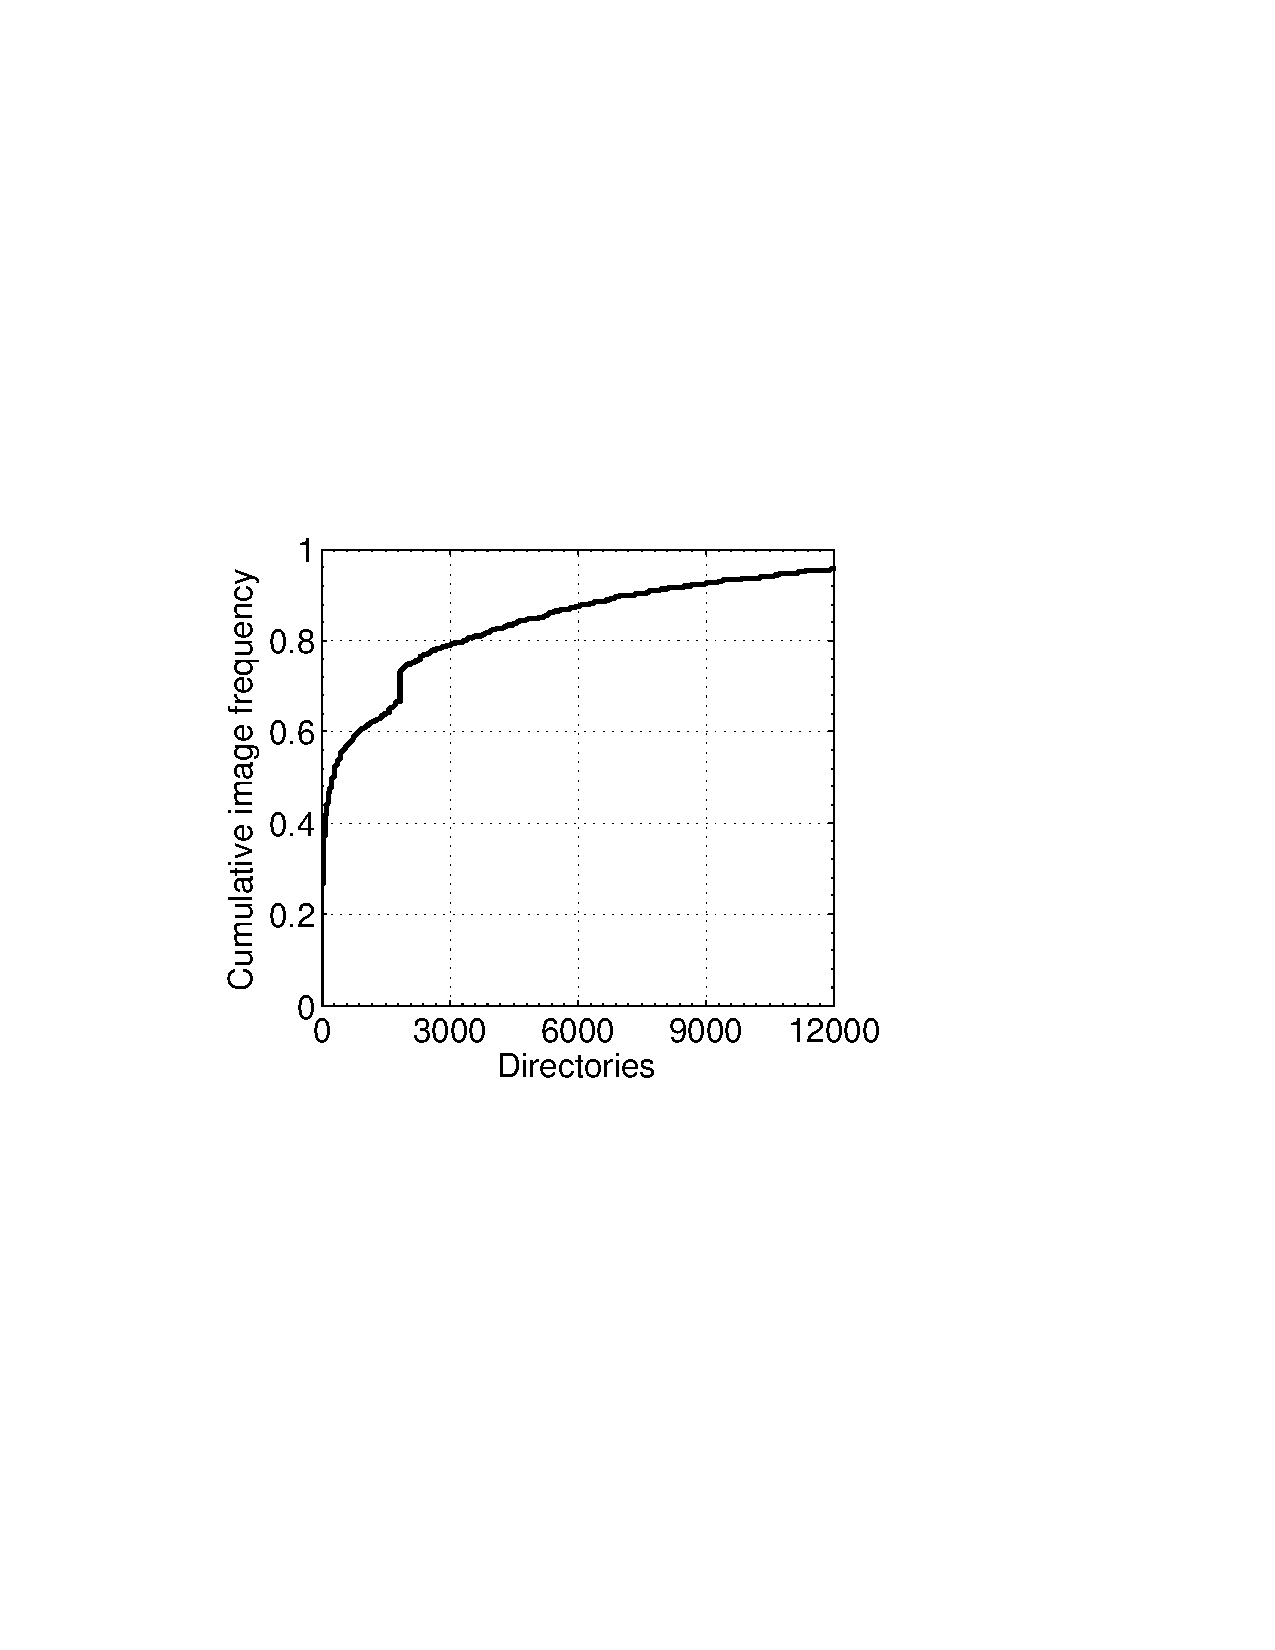
\includegraphics[width=1\textwidth]{graphs/dir.pdf}
%		\caption{CDF of images by\newline directories}
%		\label{fig-dir}
%	\end{minipage}%
%	\begin{minipage}{0.24\textwidth}
%		\centering
%		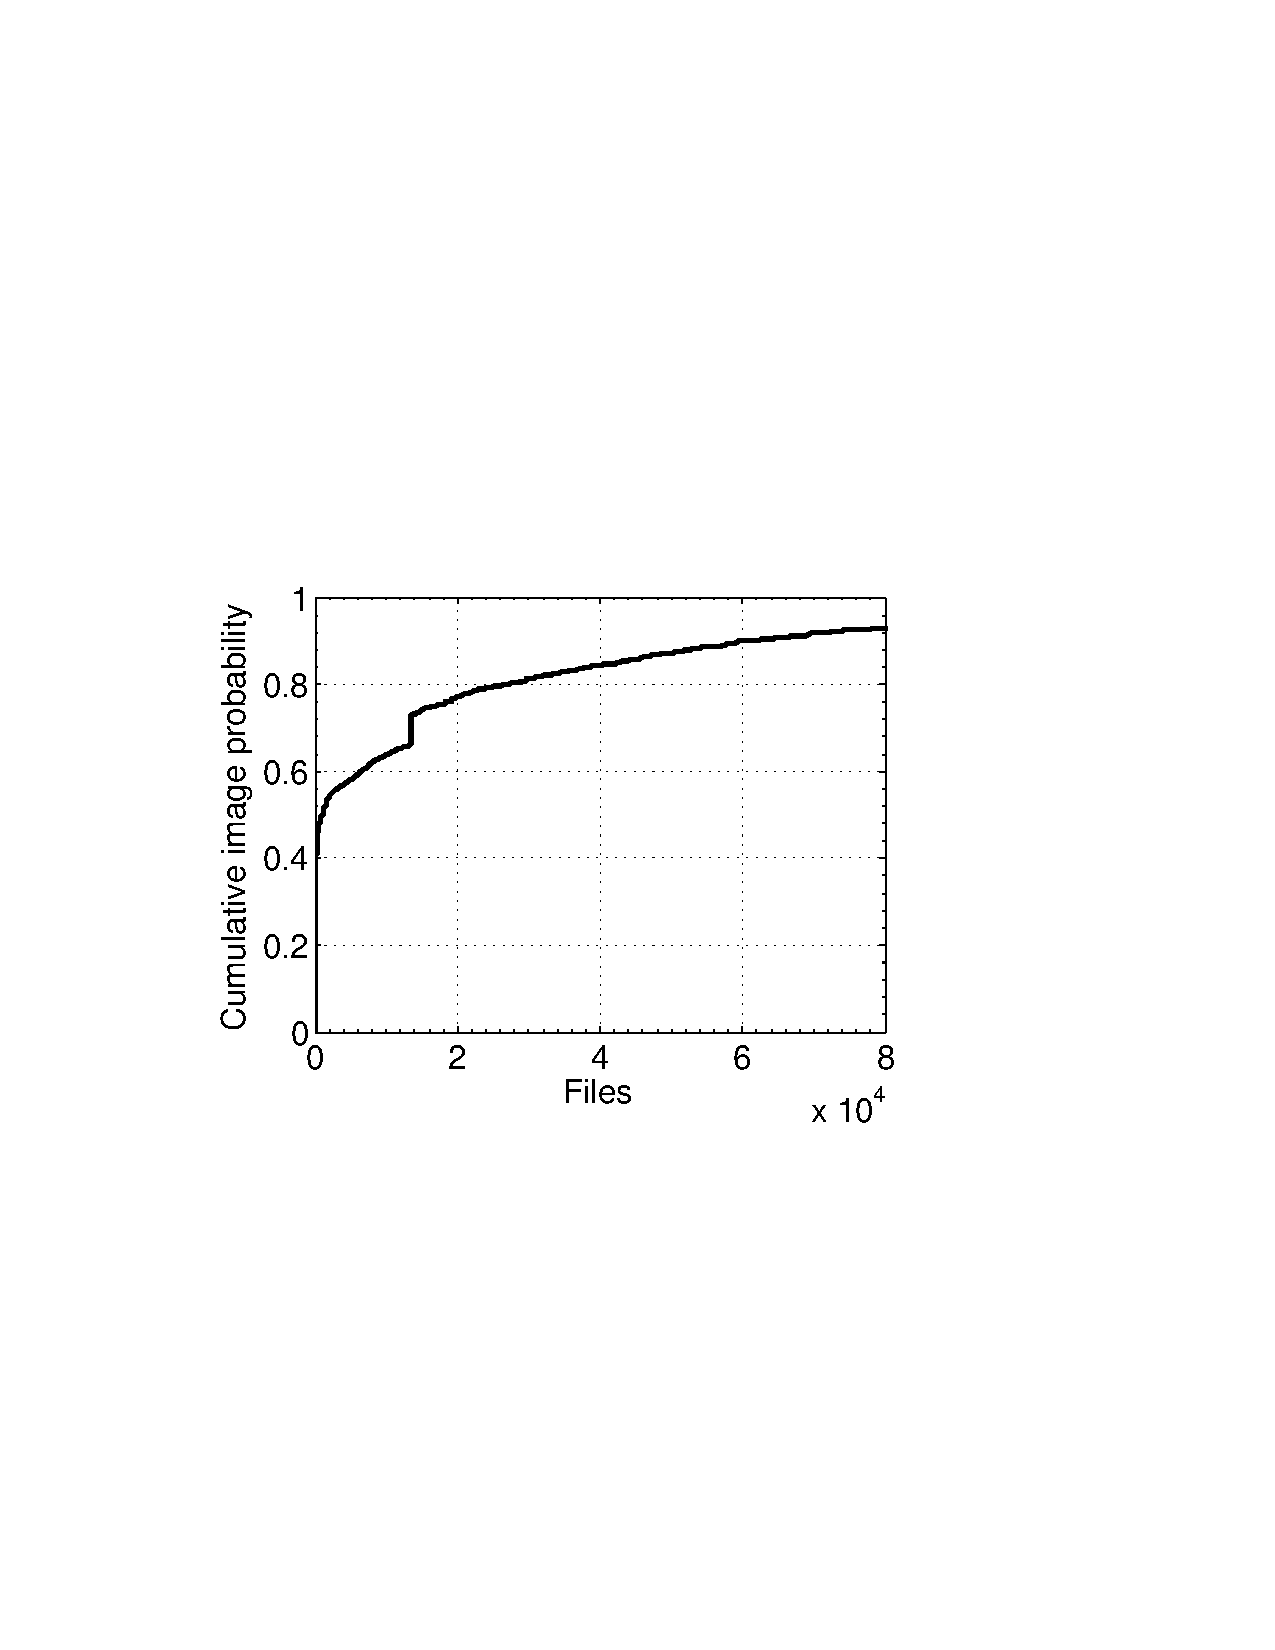
\includegraphics[width=1\textwidth]{graphs/file.pdf}
%		\caption{CDF of images by files}
%		\label{fig-file}
%	\end{minipage}
%\end{figure}

%\begin{figure}[htbp] 
%	\begin{minipage}{0.5\linewidth} 
%		\centering 
%		\includegraphics{circle} 
%		\caption{A Circle} 
%		\label{fig:circle} 
%	\end{minipage}% 
%	\begin{minipage}{0.5\linewidth} 
%		\centering 
%		\includegraphics{rectangle} 
%		\caption{A Rectangle} 
%		\label{fig:rectangle} 
%	\end{minipage} 
%\end{figure}






